 We begin by training a better patch to patch model using Q1.3 and Q1.4, like Q2.2 we also train this model from scratch (see Figure \ref{fig:Q2_4}).
 Additionally we aligned our training data using the classes from Q1.2, for example, a full-body image was always paired with a full-body image.
 This proved more effective, and we can begin to see features of the output such as clothes being changed.
 However, the results still exhibit artifacts and are lacking detail in the face. 
 
 \begin{figure}[h!]
  \begin{center}
  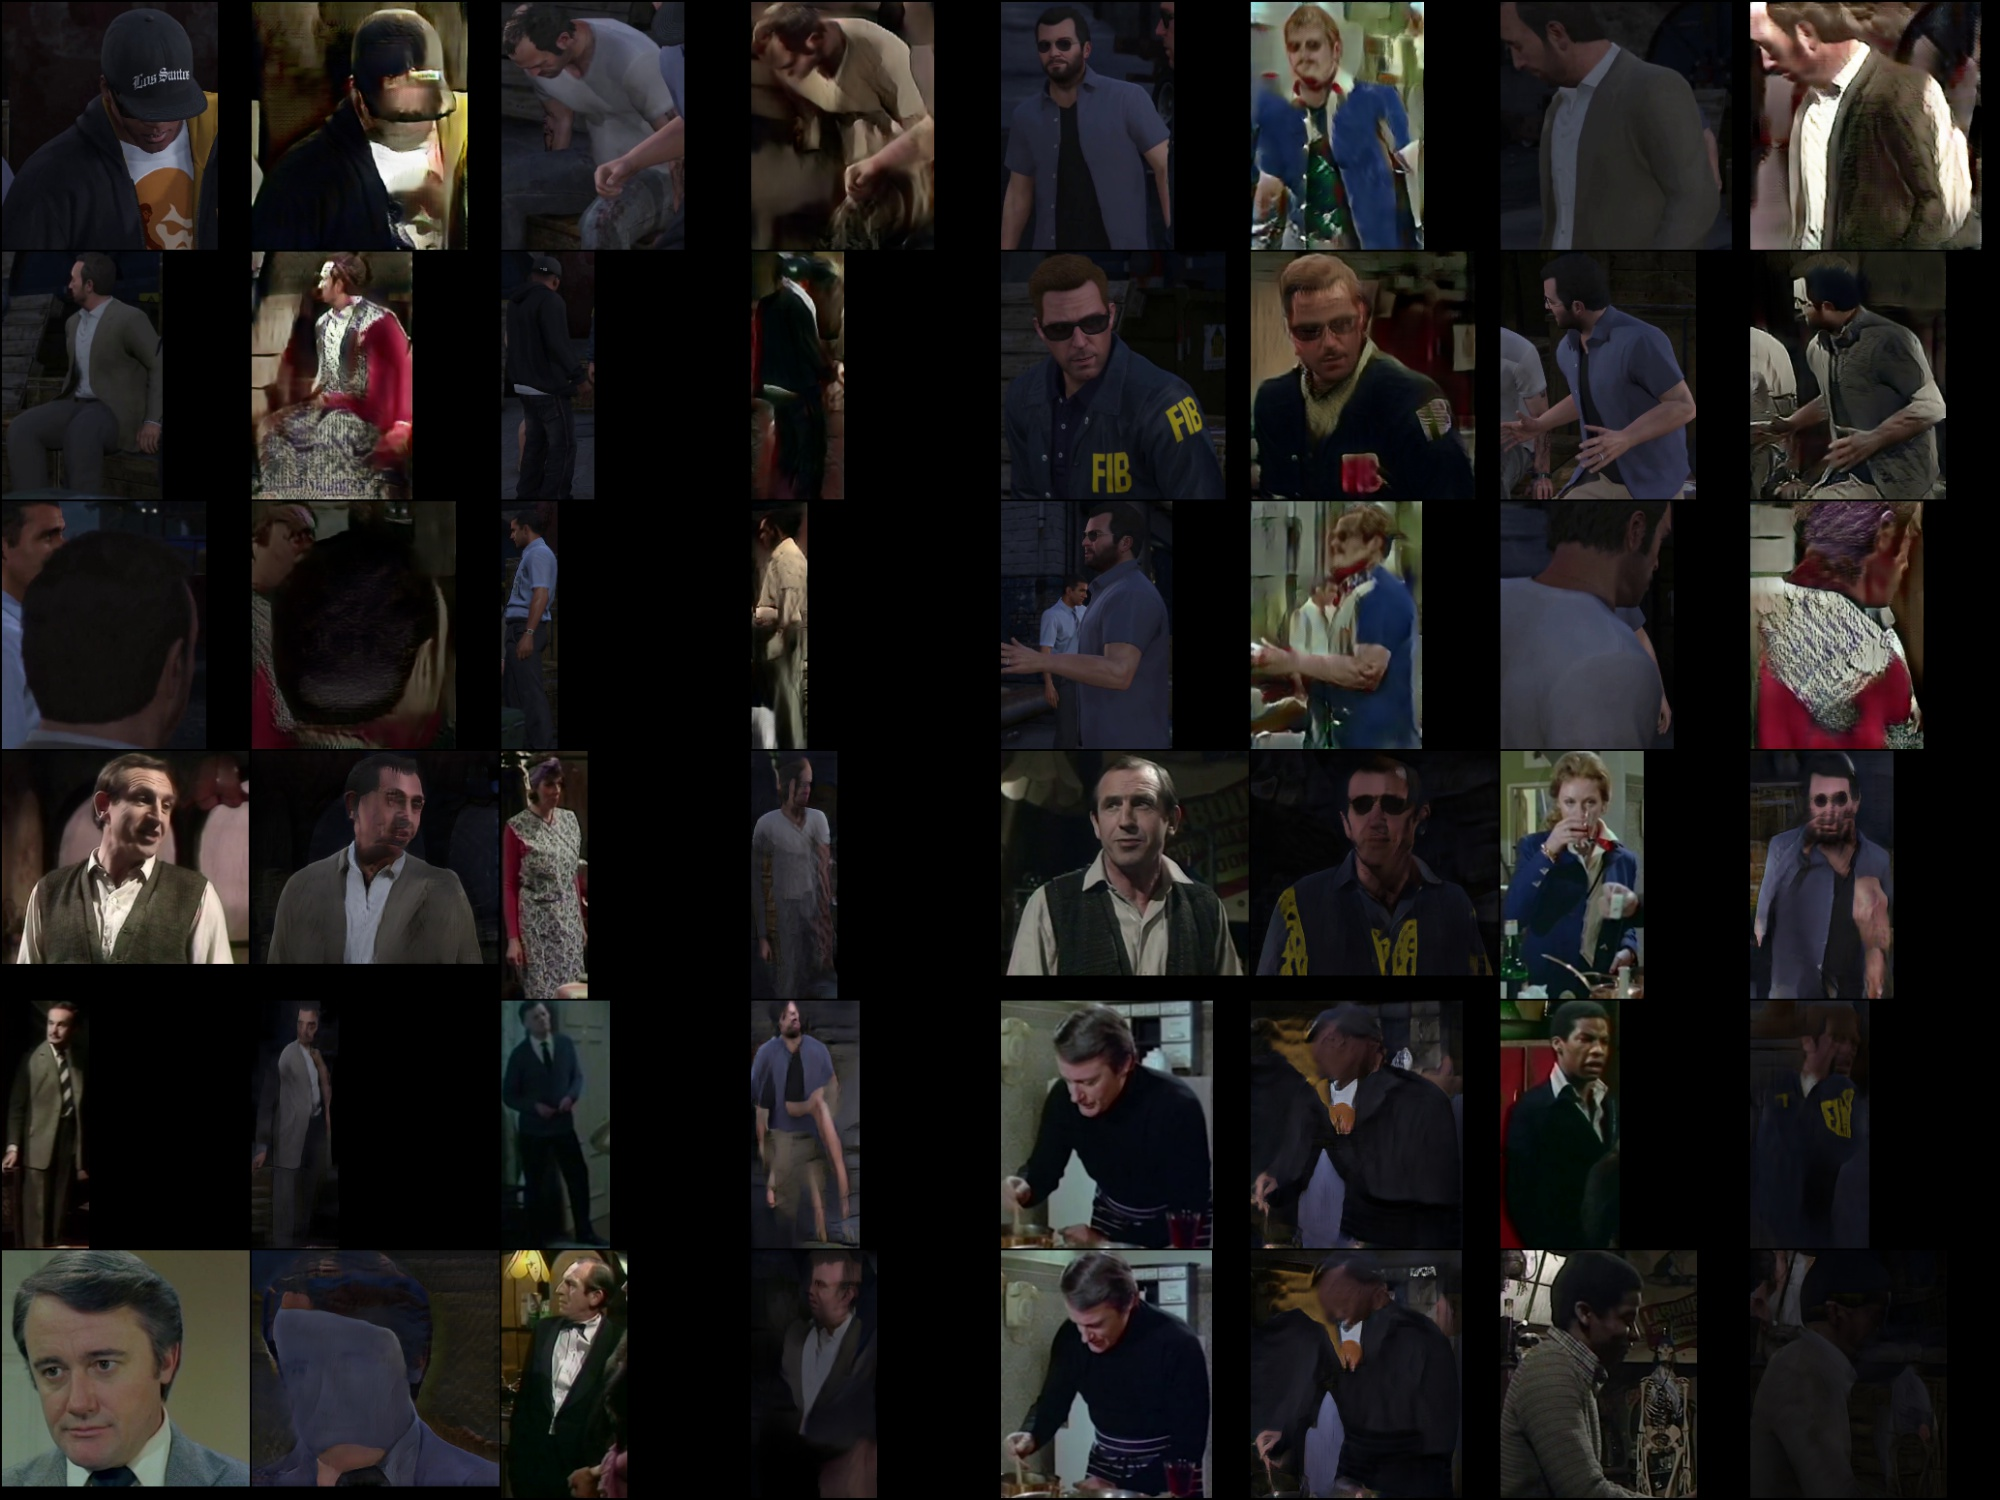
\includegraphics[scale=0.2]{Q2_3.jpg}
    \caption{Q2.3 sample of patch frames (left) and style transfer into other domain (right).}
    \label{fig:Q2_4}
  \end{center}
  \end{figure}
 
 To combine the outputs of patch model and background model we used the masks from the Mask-CNN mentioned in Q1.1.
 We continue to extract patches from the background using the Keypoint-RCNN, but also match these prediction with Mask-RCNN predictions using the Area of Intersection of bounding boxes.
 This gives us the better patch detection of Keypoint-RCNN with pixel masks from the Mask-CNN.
 These masks are used to place patches back into the background.
 